\chapter{Efficient methods to visualize finite element meshes}
\label{appendix-mesh-visualization}

Here follows the description of the methods to process and visualize large finite element meshes. The objectives for the implementation are high responsivness, comfort of use, and low memory consumption of the final mesh editor. This text with more details is also published in \cite{Benes2015}.

%----------------------------------------------------------------------------------------
%	SECTION Theoretical background
%----------------------------------------------------------------------------------------

\section{Theoretical background}

It is needed to have the model of the problem domain as a composition of individual entities, their geometry and topological connections, before a finite element mesh is generated. The model is described by its boundary and the problem domain must be discretized for further use. This process is called mesh generation \cite{XXX-2, XXX-3}. The output of a mesh generator is a finite element mesh corresponding to the input domain. The elements are the basic components and there are several types of them. The frequently used tetrahedral elements consist of four triangular faces described by three edges with the edge is made of two nodes.

It is sufficient to have only the list of nodes with their coordinates and the list of elements with references to their respective nodes for the mesh representation. Other entities (e.g. faces, edges) are usually omitted from the mesh generator output. However, the mesh editor has to handle them all, therefore, they must be created while loading the mesh. It is necessary to know all the kinds of the meshes that can be used as an input for the mesh editor implementation and especially for the design of the internal mesh representation. Meshes can be divided into several groups according to different criteria. The mesh classification is described in \cite{XXX-1}. The most basic form of mesh classification is based upon the connectivity of the mesh: structured or unstructured.

\textbf{A structured mesh}, also known as a grid, has a regular internal structure. Elements in the mesh are simply addressable due to the uniform distances between nodes. It restricts the element choices to quadrilateral in 2D or hexahedra in 3D. The regularity of the connectivity allows us to conserve space since neighborhood relationships are defined by the storage arrangement.

\textbf{An unstructured mesh} is characterized by irregular connectivity. It allows for any possible element that a solver might be able to use. When compared to the structured meshes, the storage requirements for an unstructured mesh can be substantially larger since the neighborhood connectivity must be explicitly stored.

Other mesh classification is based upon the \textbf{dimension} and the type of elements present. Depending upon the analysis type and solver requirements, meshes can be composed of one-, two- or three-dimensional elements. \textbf{Homogenous} meshes contain elements of the same type and dimension. \textbf{Hybrid} meshes are composed of elements of different type and/or dimension, e.g. tetrahedral mesh with 1D bars.

Additional classification can be made upon whether the mesh is \textbf{conformal} or not. An intersection of any two elements is either by a face, an edge or a node in conformal mesh. A non-conformal mesh contains for instance two quadrilaterals sharing two edges or two quadrilaterals sharing only a half of one edge. Non-conformal meshes are usually created during distributed generation of meshes from sub-domains and can cause issues during creation of the surface representation of non-conformal meshes. This issue is described in detail in section \ref{sec:A-implementation}.

Three-dimensional meshes can be replaced for the purpose of visualization with its surface representation. The elements (or parts of elements) that are hidden inside the volume of the mesh can be omitted. Visualization is much more efficient then. Most of the operations on entities, such as selection or setting of properties, can also be made on the mesh surface. The implementation of cuts through the volume is a problem. In order to show the entities on the cross-section, the surface representation must be regenerated each time. Making a cut is therefore a little more computationally intensive but it is outweighed by the fact that 2D surface representation is sufficient to handle any finite element mesh.

Because of the fact that the surface of both two-dimensional and three-dimensional elements is formed by either a triangle or a quadrilateral to represent the whole mesh, it is sufficient to use these two shapes. The surface representation must also include edges and vertices which the faces are formed of. The one-dimensional elements will be dealt with separately. When considering the internal representation of a mesh it is necessary to take into account the memory requirements. It should be noted that closed 3D mesh (not counting boundary elements) with homogenous structure and with $n$ elements has approximately $6n$ edges, $10n$ faces and $5n$ tetrahedral elements.

Most of the triangles and the edges will be inside the volume and can be therefore discarded after surface generation. The number of the surface entities is closely related to the geometrical shape of the domain. However, the number is significantly lower than the number of all entities for most meshes. The common operations on the mesh, e.g. to find neighboring faces, need complete topological data about the original mesh. The input file usually does not contain information about connections between elements. Therefore it must be determined while loading the mesh from the input file.

The data structure called \textbf{Winged edge} is used to store this kind of information. It is a widely used data structure in computer graphics especially for modeling practice, \cite{XXX-4-6}. It describes explicitly the geometry and topology of faces and allows fast traversing between faces, edges and vertices on the surface through a structure similar to the linked list. Traditional winged-edge data structure is represented by edge table. Each entry in the edge table contains these references: start vertex and end vertex, left face and right face, the predecessor and successor edges when traversing its left face, and the predecessor and successor edges when traversing its right face. Clockwise ordering (viewing from outside of the polyhedron) is used for traverse. Note that if the direction of the edge is changed, all entries in the table must be changed accordingly. Also, if some faces of a solid have holes, the above form of winged-edge data structure does not work. To make it work, ordering of the edges must be changed or some auxiliary edges must be added to surface representation. All these changes are difficult to implement efficiently. And this type of winged-edge data structure cannot be used for non-conformal finite element meshes. The basic composition of the winged-edge data structure that describes polygon meshes is widely used in computer graphics. However, the increased memory requirements compared to representations like the simple list of vertices and elements is the disadvantage. Moreover, the winged edge structure is based on dynamically created objects and therefore fragmentation of the memory can occur.

Figure \ref{fig:winged-edge} shows the adjusted data structure describing mesh surface based on traditional winged-edge schema, but eliminating some of its deficits. This structure is more suitable to use in finite element mesh scenario.

\begin{figure}[H]
\centering
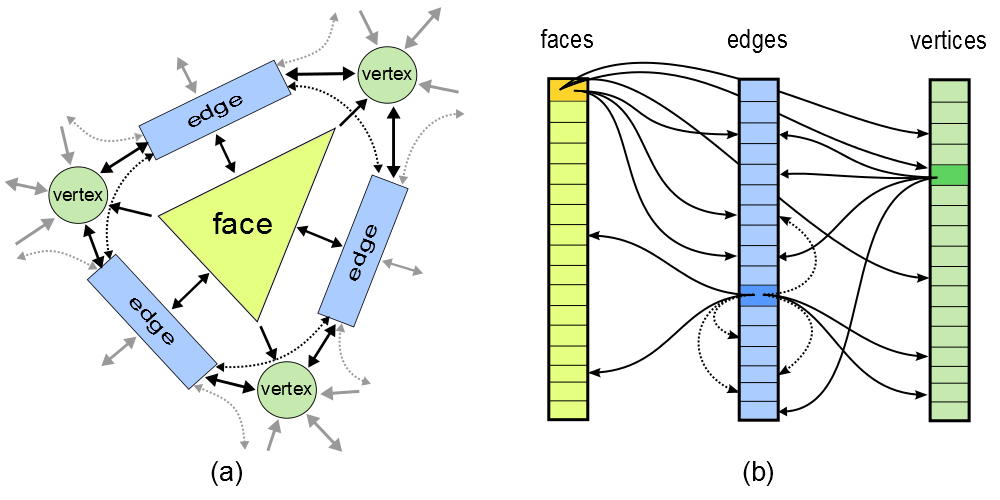
\includegraphics[width=\textwidth]{figures/appendix-mesh-visualization/figure1}
\decoRule
\caption[Winged edge data structure]{Winged edge data structure. (a) Entity dependencies. (b) Storage in lists with references.}
\label{fig:winged-edge}
\end{figure}


%----------------------------------------------------------------------------------------
%	SECTION Implementation details
%----------------------------------------------------------------------------------------

\section{Implementation details}
\label{sec:A-implementation}

All types of elements that are handled by the program are represented by the class hierarchy depicted in Figure \ref{fig:class-diagram-elements}. The common properties of all elements are accommodated in an abstract base class Element. The next level of the abstraction classifies the elements according to their spatial dimension. The particular class Beam stands for the one-dimensional element with linear approximation. The class inheriting from the Beam gains quadratic approximation by adding extra node in the middle of the line. The approximation type of other elements is distinguished by the type of their edges (a data structure describing the edge is similar to the one for 1D-elements).

\begin{figure}[H]
\centering
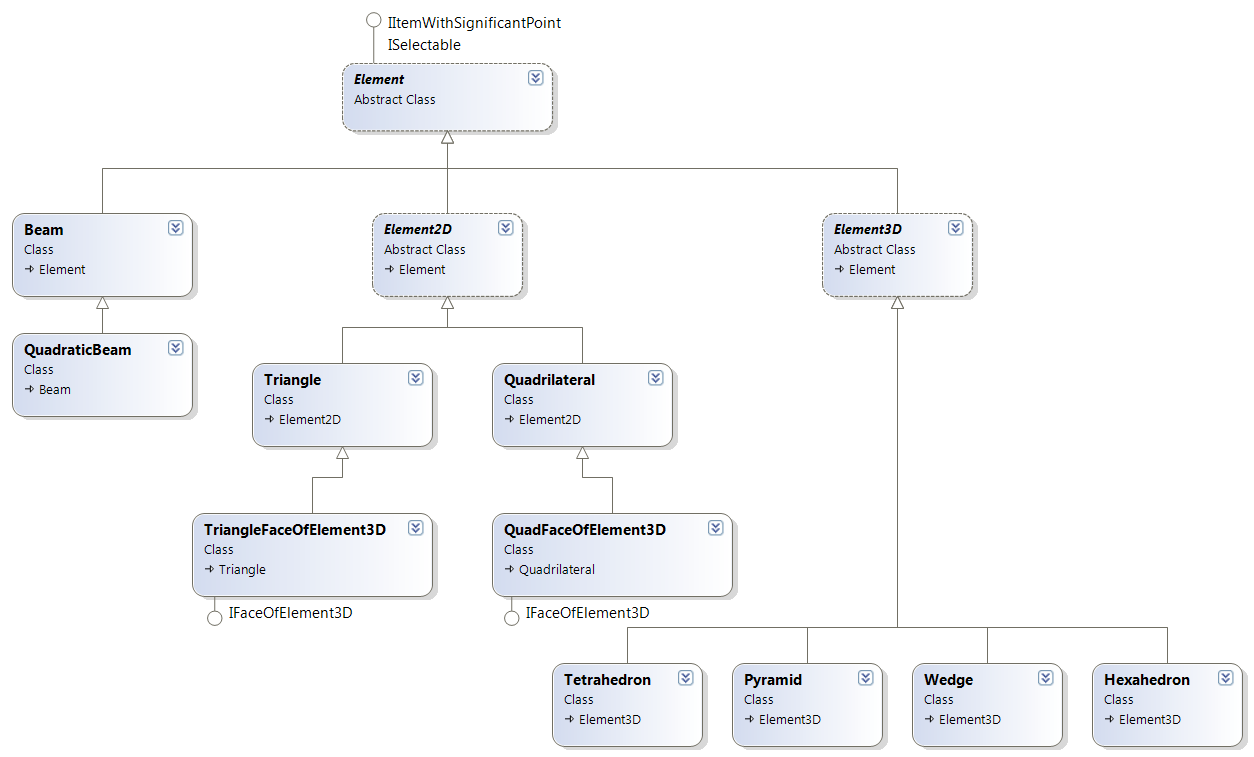
\includegraphics[width=\textwidth]{figures/appendix-mesh-visualization/figure2}
\decoRule
\caption[Class diagram of element types]{Class diagram with hierarchy of all supported element types.}
\label{fig:class-diagram-elements}
\end{figure}

The abstract base class Element2D is common for both the two-dimensional elements (triangle and quadrilateral) and faces of the three-dimensional elements (also triangles or quadrilaterals for all the widely used element types). The fact that 2D elements and faces of 3D elements can be handled in the same way allows us to implement a single generic algorithm for generation of the surface of the mesh so that the problem with hybrid meshes is hereby elegantly solved.

The 3D element face classes differ only by implementation of the interface \texttt{IFaceOfElement3D}.

\begin{Verbatim}[obeytabs,tabsize=4]
interface IFaceOfElement3D
{
	Element3D ParentElement { get; }
}
\end{Verbatim}

The interface helps to include reference to the parent 3D element at each face. This link is important for selection of elements on the mesh surface, because surface is composed, among other things, of external faces of those 3D elements that lie on the domain boundary. The adapted winged edge pattern is applied for the surface representation. All classes participating in this data structure are summarized in the class diagram in Figure \ref{fig:class-diagram-surface}.

\begin{figure}[H]
\centering
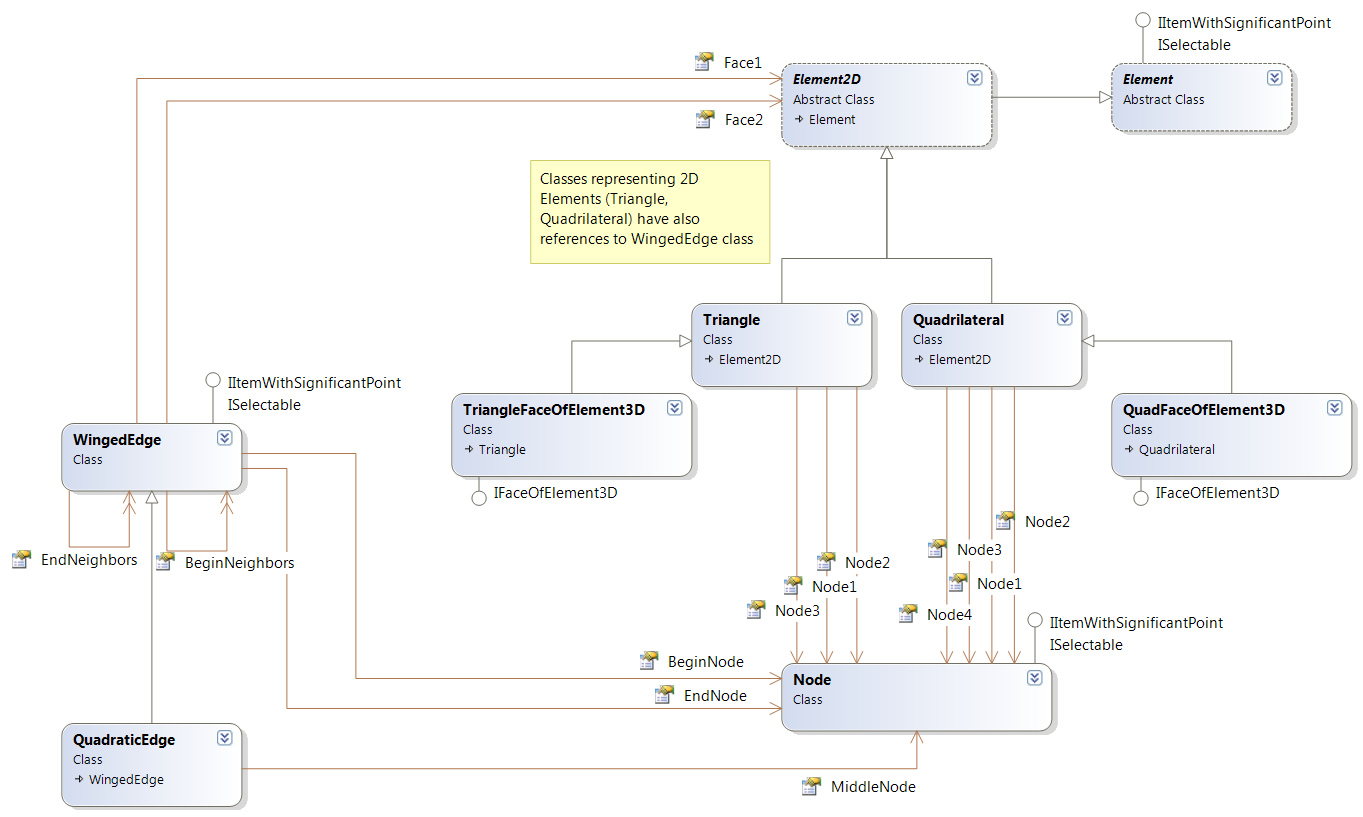
\includegraphics[width=\textwidth]{figures/appendix-mesh-visualization/figure3}
\decoRule
\caption[Class diagram of surface representation]{Class diagram with mesh surface representation.}
\label{fig:class-diagram-surface}
\end{figure}

Unlike traditional winged-edge data structure used in computer graphics in which each edge has references only to two neighboring edges, in our data structure each edge knows all its incident edges. The list of adjacent edges is tracked by every node and is shared between the node and all its neighboring edges. The ordering of edges in the list is arbitrary because in some cases there can be multiple candidates for its predecessors and successors. In this case no right ordering exists and traditional winged edge data structure used in computer graphics cannot be used. The surface representation is constructed on the fly in our single-pass algorithm. During the construction it cannot be known which edges are on the surface and what are its predecessors and successors. Therefore all adjacent edges for each node are kept in single unsorted list. To determine ordering of edges there would have to be second pass which would have significant negative impact on performance and therefore we wanted to avoid it. Moreover, for non-conform meshes there can be found no right ordering even after the surface construction.

Additionally, our approach has better memory footprint due to sharing adjacency list between node and all its neighboring edges as oppose to traditional winged edge structure. Another advantage is better performance in most common use cases of the mesh editor. Every user-triggered operation with mesh starts with selection of node or face on the mesh surface. Having direct references between each node and all its incident edges enables us quickly traverse the whole mesh surface.

Another adjustment of our data representation that differs from winged edge structure used in computer graphics is calculating and storing angle between each two neighboring faces. This enables us to implement advanced features such as finding significant edges or selection of logically related elements (e.g. on the same flat surface) as described below.

Besides the references to the begin- and end- nodes, every edge also has references to the lists of neighboring edges for each of both nodes. The lists are shared between the adjacent edges to achieve lower memory consumption. The edge also contains references to the faces on the left and on the right. This kind of linking is suitable for the majority of meshes. A problem can occur only in the non-conformal mesh processing when elements can share only a part of its surface. Visualization of this mesh can show up some artifacts caused by the fact that some internal faces do not have the adjacent counterparts and thus cannot be paired off. Another problem shows up when some elements have only one edge in common. In that case, the edge can be shared by more than two faces and the winged edge data structure cannot capture properly this situation. However, these are rare cases and do not render the program unusable.

%----------------------------------------------------------------------------------------
%	SUB-SECTION Data structures overview
%----------------------------------------------------------------------------------------

\subsection{Data structures overview}

The modified winged-edge data structure was used to describe the internal surface representation of a mesh. Instead of references to the left and the right adjacent edges, each node has reference to the list of all edges that begin or end at this node. The references to these lists are also contained in each winged-edge object. This approach allows representing the meshes with some abnormalities or non-conformal meshes in where it is impossible to determine which edge is the left and which is the right. Other characteristics of the winged-edge data structure remain the same. Each edge has references to the left and the right adjacent faces. Each face has references to its nodes, edges and the parent 3D element. The elements need to have references only to its nodes, because not every element is on the mesh boundary and so it does not need to have reference to surface objects. Every operation on the mesh, such as selection, begins with either a face or a node on the surface. Other entities are found by searching through the links in the winged edge data structure. Figure \ref{fig:data-structure-mesh} shows data lists used in the mesh editor.

\begin{figure}[H]
\centering
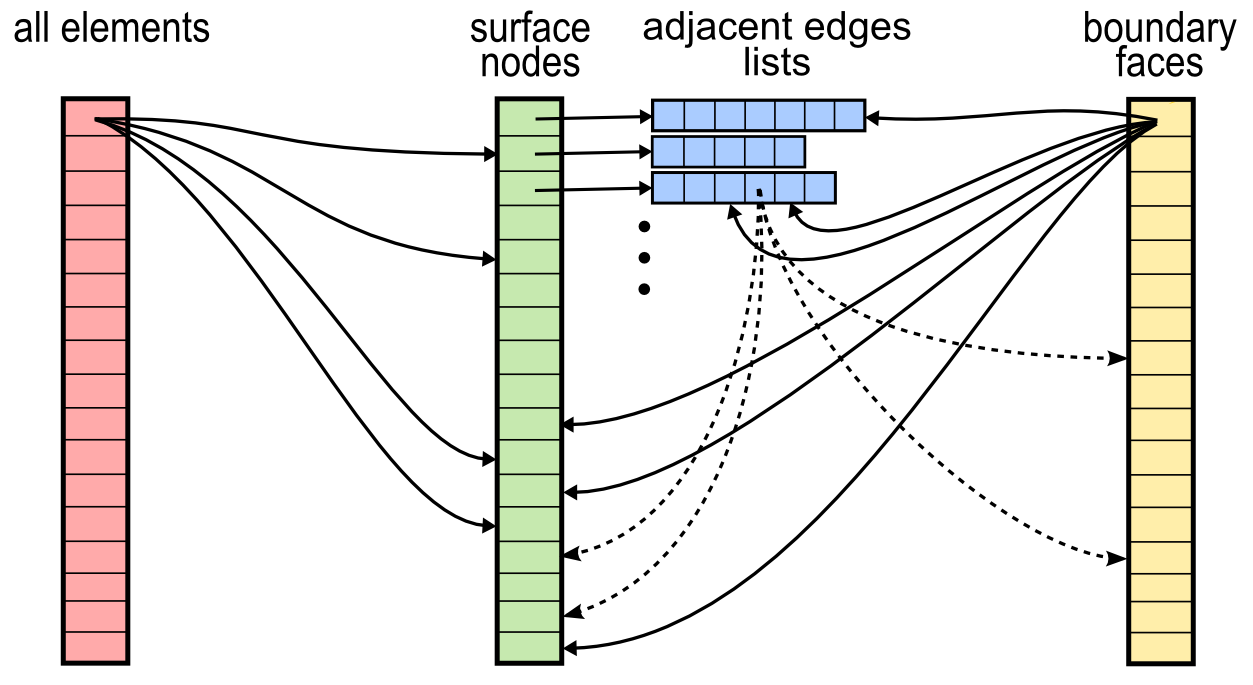
\includegraphics[width=\textwidth]{figures/appendix-mesh-visualization/figure4}
\decoRule
\caption[Data structure overview]{Diagram with data structure overview.}
\label{fig:data-structure-mesh}
\end{figure}

Memory requirements of each entity object are summarized in Figure \ref{fig:surface-rep-memory}. The overall memory consumption depends highly on the mesh topology and on the ratio of the number of surface elements to the total number of elements. This ratio decreases with the growing size of the mesh (or the element density) because the total number of elements increases with cube of the size of mesh, unlike the number of surface elements which increases with square of the mesh size.

\begin{figure}[H]
\centering
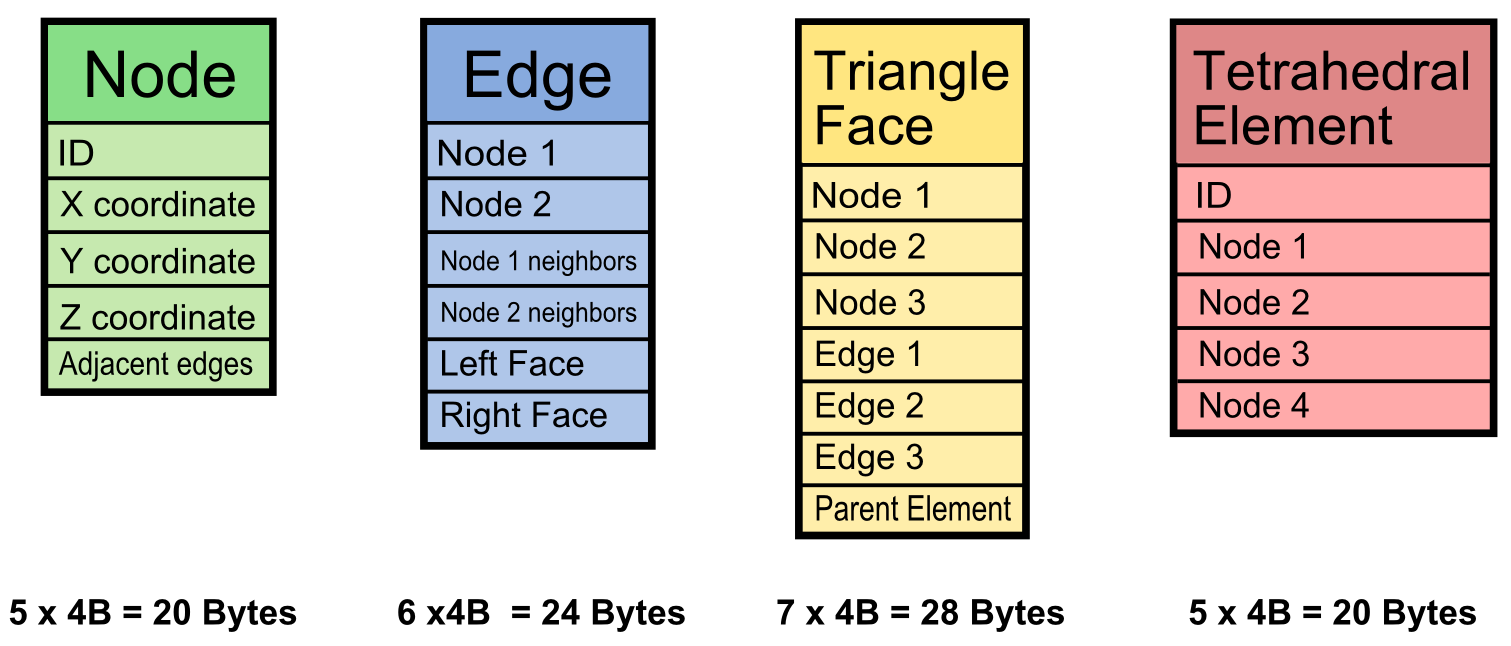
\includegraphics[width=\textwidth]{figures/appendix-mesh-visualization/figure5}
\decoRule
\caption[Memory consumption of surface representation]{Memory consumption of surface entity objects.}
\label{fig:surface-rep-memory}
\end{figure}

%----------------------------------------------------------------------------------------
%	SUB-SECTION Surface representation construction
%----------------------------------------------------------------------------------------

\subsection{Surface representation construction}